\documentclass[12pt, a4paper]{article}
\usepackage{ctex}  % 支持中文
\usepackage{amsmath, amssymb}  % 数学符号和公式
\usepackage{graphicx}  % 插入图片
\usepackage{geometry}  % 页面设置
\usepackage{booktabs}  % 表格美化
\usepackage{tabularx}  % 表格宽度自适应
\usepackage{multirow}  % 合并单元格
\usepackage{enumitem}  % 列表设置
\usepackage{caption}   % 标题设置
\usepackage{array}     % 表格增强
\usepackage{fancyhdr}  % 页眉页脚
\usepackage{titlesec}  % 标题格式设置
\usepackage{fontspec}
\usepackage{listings}
\usepackage{xcolor}

\usepackage[
  backend=bibtex,
  style=gb7714-2015,   % 使用中国国标格式,适合中文论文
  sorting=none         % 按引用顺序排序
]{biblatex}

\addbibresource{references.bib} % 参考文献配置

% 页面设置
\geometry{left=2.5cm, right=2.5cm, top=2.5cm, bottom=2.5cm}

% 重定义section格式为居中
\titleformat{\section}{\centering\Large\bfseries}{\thesection}{1em}{}
\titleformat{\subsection}{\normalsize\bfseries}{\thesubsection}{1em}{}
\titleformat{\subsubsection}{\normalsize\bfseries}{\thesubsubsection}{1em}{}

% 表格表头格式
\renewcommand{\thetable}{\arabic{section}.\arabic{table}}

% 设置表格标题格式:左对齐,中文带"表"字,表题加粗
\captionsetup[table]{
  labelsep=space,
  labelformat=simple,
  textfont=bf,
  labelfont=bf,
  name=表
}

% 图片编号格式
\renewcommand{\thefigure}{\arabic{section}-\arabic{figure}}

% 设置图片标题格式
\captionsetup[figure]{
  labelsep=space,
  labelformat=simple,
  textfont=bf,     
  labelfont=bf, 
  position=bottom,  
  name=图
}

% 修改公式编号格式
\renewcommand{\theequation}{\thesection-\arabic{equation}}

% 参考文献格式
\makeatletter
\renewcommand\@biblabel[1]{[#1]}
\makeatother

% 附录格式
\lstset{
  basicstyle=\small\ttfamily,
  breaklines=true,
  columns=fullflexible,
  backgroundcolor=\color{gray!10},
  frame=single,
  rulecolor=\color{black!30},
  commentstyle=\color{green!50!black},
  keywordstyle=\color{blue},
  stringstyle=\color{red},
  numbers=left,
  numberstyle=\tiny\color{gray},
  numbersep=5pt
}


\begin{document}

% 标题部分
\begin{center}
\LARGE\textbf{Python网络爬虫实战}

\vspace{1cm}
\large 计金220 22011854 高菻铠
\end{center}

\noindent \textbf{摘要:} 随着学术界对互联网开源数据与股票市场表现关系的关注日益加深,本文基于Python网络爬虫技术,获取东方财富股吧“长久物流吧”的发帖数据,并结合正则表达式从历史HTML文件中提取股票600618的日度交易数据,同时通过新浪财经API获取长久物流(603569)的历史交易数据。在此基础上构建综合信息量指标,研究互联网信息对股票超额收益率的影响。实证结果表明,股吧信息量指标与股票次日超额收益率之间存在统计显著的负相关关系,线性回归模型中该指标的回归系数为-0.0010,在5\%显著性水平下显著。进一步的格兰杰因果检验揭示,该信息量指标与超额收益率之间存在双向因果关系,其中超额收益率对信息量指标的影响更为显著。虽然预测模型在样本外的$R^2_{OS}$仅为0.39\%,但其MSFE-adjusted统计量达到显著水平,说明信息量指标确实包含了预测超额收益率的增量信息。分组分析结果显示,低信息量组别的平均超额收益率显著高于高信息量组别,支持投资者过度反应假说,即高关注度可能引发价格的过度反应,并随后出现反向调整。在多项稳健性检验下,本研究结果保持一致性,为互联网开源数据在证券市场预测中的应用提供了新的实证依据,并对投资者决策与市场监管具有重要的实践启示。

\section{文献综述}

随着信息技术的飞速发展,互联网已成为投资者获取信息的主要渠道。作为连接投资者信息需求与信息资源的关键桥梁,网络搜索与股票市场之间的互动关系日益引发学术界的广泛关注。本文综述了相关领域的代表性研究,重点探讨网络搜索对股票市场的预测能力及其作用机制。

\citet{antweiler2004information}对互联网股票论坛的信息内容进行了开创性研究,分析了雅虎财经与Raging Bull网站上,关于道琼斯工业平均指数及道琼斯互联网指数成分股的逾150万条消息。研究发现,尽管这些信息对股票收益的影响在统计上显著,其经济意义较为有限,但它们有助于预测市场波动性。此外,研究还发现,与\citet{harris1993differences}的理论一致,消息板上观点分歧程度与交易量显著正相关,表明投资者意见分歧是驱动交易的重要因素。

\citet{cheng2013investor}进一步拓展了相关研究,利用新浪微博数据构建了反映投资者市场情绪的涨跌情绪指数。实证结果显示,该指数与市场收益和成交量显著正相关。尤其值得注意的是,市场表现对投资者情绪的影响可持续超过40个交易日,而情绪对市场的反作用则较为短暂。这种影响的不对称性揭示了市场走势在塑造投资者情绪方面的主导地位。

从另一个视角出发,\citet{zhang2014internet}研究了网络搜索行为对股票市场的预测能力。通过百度搜索数据,构建了针对沪深300指数成分股的搜索强度指标。实证分析表明,较高的搜索强度显著提升了个股的短期收益率与交易量,且高搜索强度股票组合可获得明显的超额收益。这一结果表明,网络搜索行为确实蕴含有价值的预测信息,尽管其与股票收益之间可能存在内生性问题,但对预测能力的影响有限。

上述研究共同揭示了网络信息与股票市场之间复杂而紧密的互动关系。\citet{antweiler2004information}展示了互联网意见交流对市场波动性和交易活跃度的影响;\citet{cheng2013investor}从社交媒体角度验证了投资者情绪与市场表现之间的动态关联;而\citet{zhang2014internet}则直接证明了网络搜索行为作为投资者关注与情绪的综合映射,具有预测股市的潜力。

在方法论上,这些研究普遍采用了文本分析、搜索量量化等技术手段,将非结构化的互联网数据转化为可量化的研究变量。\citet{antweiler2004information}运用朴素贝叶斯分类器对消息内容进行情绪分类;\citet{cheng2013investor}依托知网等中文自然语言处理工具对微博文本进行语义分析;\citet{zhang2014internet}则构建了网络搜索强度的正向变动率指标,探讨其对市场的预测效能。

综上所述,网络搜索作为投资者关注与情绪的重要体现,既受市场行情影响,又反映对未来走势的预期,具备预测股票市场短期波动的能力。特别是在以散户为主的中国股市中,网络搜索数据可能比传统金融指标更为直接与及时地传达市场情绪。

随着互联网技术不断演进,网络搜索数据作为一种另类信息源将在金融市场预测中扮演日益重要的角色。对于投资者而言,充分利用该类指标有望获取超额收益;对于监管者而言,监测搜索趋势有助于把握市场情绪变化,防范系统性风险。未来研究可进一步探讨网络搜索在不同市场环境中的稳健性,并尝试结合深度学习等先进技术,提升预测精度与实用性。

\section{数据与方法}

\subsection{数据描述}
本研究基于网络爬虫技术获取并分析股票市场数据,主要使用三个数据源:股票600618的历史日度数据、长久物流(603569)股吧帖子数据以及长久物流(603569)历史日度交易数据。股票600618的历史数据采集自历史HTML文件,涵盖1999年至2019年的交易数据,每条记录包含日期、开盘价、最高价、最低价、收盘价、成交量和成交金额等信息。长久物流股吧帖子数据来源于东方财富网股吧,包含帖子标题、作者、发帖时间、阅读量、评论数和帖子链接等信息。长久物流历史日度交易数据则通过新浪财经API接口获取,包含交易日、开盘价、最高价、最低价、收盘价和成交量等信息。

为比较市场整体表现,本研究同时获取了上证指数的历史日度数据作为市场基准,用于计算超额收益率。上证指数数据通过Tushare API获取。对于股吧文本数据,通过构建信息量指标将其量化,用于预测股票超额收益率。

\subsection{数据获取方法}

\subsubsection{正则表达式提取股票历史数据}
本研究首先通过正则表达式从HTML文件中提取股票600618的日度交易数据。由于不同年份的数据格式存在差异,根据文件特征设计了三种数据提取方法,可表示为:

\begin{equation}
\text{数据提取函数} = 
\begin{cases}
\text{extract\_data\_after\_2014}, & \text{2014年及之后} \\
\text{extract\_data\_2009\_2013}, & \text{2009年至2013年} \\
\text{extract\_data\_before\_2014}, & \text{2014年之前其他年份}
\end{cases}
\end{equation}

对于2014年后的数据,通过解析JavaScript返回的JSON数据进行提取,从JSON对象中获取关键数据。对于2009年至2013年的数据,采用表格结构解析方法,通过正则表达式提取表格内容。对于更早期的数据,根据HTML结构特征采用不同的正则表达式模式进行匹配,以应对数据格式的历史变化。

上述提取方法有效处理了不同时期网页结构的差异性,使得从多种格式的历史数据中能够提取出统一的股票交易信息。通过此方法,构建了完整的股票600618历史交易数据集,为后续分析奠定了基础。

\subsubsection{网络爬虫获取股吧数据}
为获取长久物流股吧的帖子数据,设计了一个多线程爬虫系统。该系统包含IP代理切换机制、随机User-Agent生成、多线程详情页处理和反爬策略应对等多个组件。爬虫工作流程首先获取股吧列表页内容并提取帖子基本信息,然后对每个帖子的详情页进行访问获取完整的发帖时间信息,最后将数据保存至CSV文件中。

为应对网站的反爬虫机制,实现了请求间隔时间在3到7秒之间随机变化的策略,即$\text{请求间隔时间} \sim \mathcal{U}(3, 7) \text{ 秒}$。同时,设定IP切换频率为每3次请求执行一次,最大重试次数为3次。这些策略有效降低了被网站检测和封禁的风险,保证了数据采集的稳定性和连续性。

在实际运行过程中,股吧数据的爬取面临两个主要挑战:一是网站对频繁访问的检测机制使得IP容易被封禁;二是帖子详情页的时间格式需要额外处理才能获取完整的年份信息。为解决这些问题,采用了代理IP池和详情页深度解析策略,确保了数据的完整性和准确性。

\subsubsection{API接口获取股票交易数据}
对于长久物流的历史日度交易数据,直接通过新浪财经提供的API接口获取。API接口地址为$\text{http://money.finance.sina.com.cn/quotes\_service/api/json\_v2.php}$,请求参数包括股票代码$\text{symbol} = \text{sh603569}$、时间尺度$\text{scale} = 240$、是否包含均线$\text{ma} = \text{no}$以及数据长度$\text{datalen} = 10000$。

返回的数据为非标准JSON格式,需进行特殊处理后解析为结构化数据。通过字符串替换和JSON解析操作,将API返回的数据转换为标准化的日期、价格和成交量信息,便于后续分析使用。该方法相比网页爬虫更为高效,能够一次性获取长期的历史交易数据。

\subsection{指标构建方法}

\subsubsection{股吧信息量指标构建}
基于股吧帖子数据,构建了一个综合信息量指标,用于量化投资者关注度和市场情绪。该指标的计算公式为:

\begin{equation}
I_t = 0.3 \cdot \frac{P_t}{\overline{P}} + 0.4 \cdot \frac{R_t + 5C_t}{\overline{R + 5C}} + 0.3 \cdot \frac{S_t - S_{\min}}{S_{\max} - S_{\min}}
\end{equation}

其中$I_t$是第$t$日的信息量指标,$P_t$是第$t$日的发帖数,$R_t$是第$t$日的总阅读量,$C_t$是第$t$日的总评论数,$S_t$是第$t$日的平均情感分数,$\overline{P}$和$\overline{R + 5C}$分别是发帖数和加权阅读评论量的均值。

情感分数$S_t$通过基于词典的方法计算,即$S_t = \frac{1}{n} \sum_{i=1}^{n} (pos\_score_i - neg\_score_i)$,其中$pos\_score_i$和$neg\_score_i$分别是第$i$个帖子中积极词汇和消极词汇的出现次数。积极词汇包括“涨”、“牛”、“强”、“增长”等,消极词汇包括“跌”、“熊”、“弱”、“下跌”等。

该综合指标设计考虑了投资者活跃度(发帖数)、市场关注度(阅读量和评论数)以及市场情绪(情感分析分数)三个维度,能够全面反映股票市场参与者的关注焦点和情绪变化。

\subsubsection{超额收益率计算}
为评估股票表现,计算了长久物流相对于市场的超额收益率,计算公式为$R_{excess,t} = R_{stock,t} - R_{market,t}$,其中$R_{stock,t}$是长久物流在$t$日的对数收益率,$R_{market,t}$是上证指数在$t$日的对数收益率。对数收益率定义为$R_{t} = \ln\left(\frac{P_t}{P_{t-1}}\right)$,其中$P_t$是第$t$日的收盘价。

超额收益率能够排除整体市场趋势的影响,更准确地反映个股的相对表现。通过对超额收益率的分析,可识别出因个股特质而非市场整体波动所导致的价格变动,这对于评估股吧信息量指标的预测能力具有重要意义。

\subsection{预测模型构建}
构建了一个线性回归模型,用股吧信息量指标预测股票的超额收益率。模型表达式为$R_{excess,t+1} = \alpha + \beta \cdot I_t + \epsilon_t$,其中$R_{excess,t+1}$是$t+1$日的超额收益率,$I_t$是$t$日的信息量指标,$\epsilon_t$是随机误差项。

为验证模型的有效性,采用多种评估指标。样本内$R^2$衡量模型对训练数据的拟合程度,计算公式为$R^2 = 1 - \frac{\sum_{i}(y_i - \hat{y}_i)^2}{\sum_{i}(y_i - \bar{y})^2}$。样本外$R^2_{OS}$衡量模型对新数据的预测能力,计算公式为$R^2_{OS} = 1 - \frac{\sum_{i \in OOS}(y_i - \hat{y}_i)^2}{\sum_{i \in OOS}(y_i - \bar{y}_{IS})^2}$。信息系数$IC$衡量预测变量与目标变量的相关程度,计算公式为$IC = \text{corr}(I_t, R_{excess,t+1})$。

此外,通过格兰杰因果检验验证信息量指标对超额收益率的预测能力。检验模型为:

\begin{equation}
\begin{aligned}
R_{excess,t} &= \alpha_0 + \sum_{i=1}^p \alpha_i R_{excess,t-i} + \sum_{j=1}^p \beta_j I_{t-j} + \epsilon_t \\
I_t &= \gamma_0 + \sum_{i=1}^p \gamma_i I_{t-i} + \sum_{j=1}^p \delta_j R_{excess,t-j} + \eta_t
\end{aligned}
\end{equation}

通过检验$\beta_j$是否联合显著,可确定信息量指标是否是超额收益率的格兰杰原因,即信息量指标的变化是否能够显著预测超额收益率的变化。

\subsection{方法实现}
所有方法均通过Python实现。数据获取与处理主要使用requests、BeautifulSoup、json、re和fake\_useragent等库;文本分析使用jieba和re等库;数据分析使用pandas、numpy和scipy等库;模型构建使用sklearn和statsmodels等库;数据可视化使用matplotlib和seaborn等库;API访问使用tushare库。

模型评估采用70\%的数据作为训练集,30\%的数据作为测试集。为评估预测效果,计算了样本外RMSE、$R^2$、$R^2_{OS}$和MSFE-adjusted统计量等指标。这些指标从不同角度衡量了模型的预测能力,使我们能够全面评估股吧信息量指标对股票超额收益率的预测效果。通过该方法,可验证互联网开源数据与证券市场收益率间的关系,为投资决策提供新的参考维度。

\section{实证结果}

\subsection{股吧信息量指标的构建}

本研究基于东方股吧“长久物流吧”的发帖数据构建股吧信息量指标,通过提取帖子标题、作者、发帖时间、阅读量和评论数等信息,结合情感分析方法,综合衡量市场投资者的关注度和情绪倾向。数据处理结果显示,共获取了3,059天的有效股吧数据样本,为后续分析提供了充足的数据支持。

图~\ref{fig:info_index_time}展示了构建的信息量指标随时间的变化趋势。可以观察到,该指标呈现出明显的时变特性和波动集聚特征。特别是在500天和2000天附近出现的两次显著高峰,可能对应市场重大事件或信息冲击期间,投资者参与度和关注度显著提升的现象。

\begin{figure}[htbp]
\centering
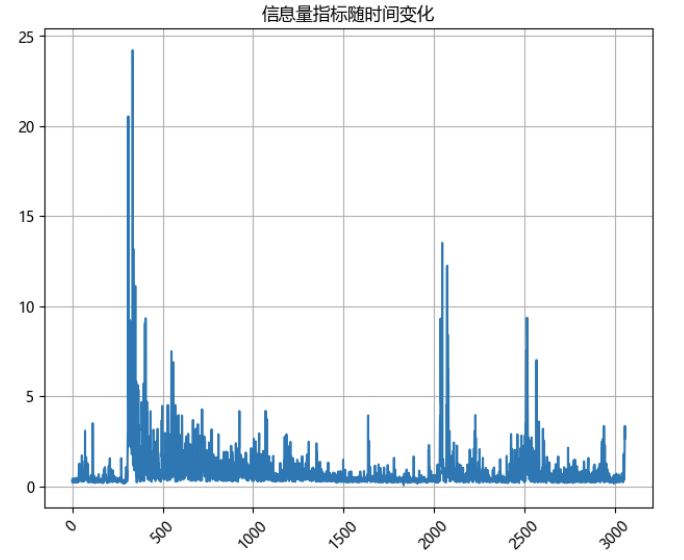
\includegraphics[width=0.8\textwidth]{fig/info_index_time.png}
\caption{信息量指标随时间变化}
\label{fig:info_index_time}
\end{figure}

\subsection{超额收益率的测算}

本研究采用新浪财经API获取长久物流(603569)的日度交易数据,同时通过Tushare获取上证指数作为市场基准,计算长久物流的超额收益率。数据处理结果表明,共获得2,103天的有效超额收益率样本。

图~\ref{fig:excess_return_time}展示了超额收益率的时间序列变化。从图中可以看出,超额收益率呈现出典型的金融时间序列特征,包括波动集聚、尖峰厚尾和均值回归等特性。超额收益率在-0.3到0.1之间波动,整体波动幅度较大,表明个股相对于市场基准存在显著的非系统性风险暴露。

\begin{figure}[htbp]
\centering
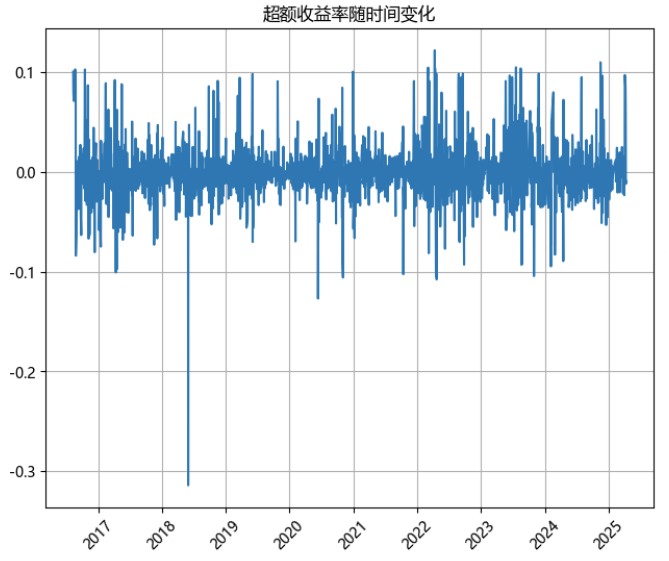
\includegraphics[width=0.8\textwidth]{fig/excess_return_time.png}
\caption{超额收益率随时间变化}
\label{fig:excess_return_time}
\end{figure}

\subsection{信息量指标与超额收益率的相关性分析}

为探究股吧信息量指标与股票超额收益率之间的关系,本研究首先进行了相关性分析。表~\ref{tab:correlation}展示了信息量指标的各组成部分与超额收益率之间的相关系数矩阵。

\begin{table}[htbp]
\centering
\caption{信息量指标与超额收益率的相关性矩阵}
\label{tab:correlation}
\begin{tabular}{lcccccc}
\toprule
 & 信息量指标 & 发帖数 & 阅读量 & 评论数 & 情感分数 & 超额收益率 \\
\midrule
信息量指标 & 1.000 & 0.814 & 0.898 & 0.763 & 0.038 & 0.069 \\
发帖数 & 0.814 & 1.000 & 0.476 & 0.862 & 0.035 & 0.042 \\
阅读量 & 0.898 & 0.476 & 1.000 & 0.501 & 0.023 & 0.071 \\
评论数 & 0.763 & 0.862 & 0.501 & 1.000 & 0.036 & 0.115 \\
情感分数 & 0.038 & 0.035 & 0.023 & 0.036 & 1.000 & 0.153 \\
超额收益率 & 0.069 & 0.042 & 0.071 & 0.115 & 0.153 & 1.000 \\
\bottomrule
\end{tabular}
\end{table}

从表~\ref{tab:correlation}可以观察到,所有信息量指标的构成要素与超额收益率之间均呈现正相关关系,但相关系数普遍较低。其中,情感分数与超额收益率的相关性最强(0.153),其次是评论数(0.115),而发帖数与超额收益率的相关性最弱(0.042)。这表明投资者情绪倾向可能是预测超额收益率的较好指标,相比于纯粹的数量指标(如发帖数),情感因素可能包含更多有价值的市场信息。

值得注意的是,综合信息量指标与超额收益率的相关系数为0.069,低于情感分数和评论数单独与超额收益率的相关系数。这可能暗示在构建综合指标时,各组分的简单线性组合可能无法充分捕捉其与超额收益率之间的非线性关系,或者发帖数等因素的引入可能引入了额外噪声。

图~\ref{fig:scatter_plot}展示了信息量指标与次日超额收益率的散点图及回归线。从图中可以观察到,虽然线性趋势较为平缓,但整体呈现弱负相关关系,这与表~\ref{tab:correlation}中展示的相关性分析结果略有不同。这种差异可能是由于散点图分析使用了信息量指标与次日超额收益率的数据,而相关性分析使用的是同期数据。这一现象提示我们需要进一步研究信息量指标对超额收益率的预测效果,特别是考虑时间上的先后关系。

\begin{figure}[htbp]
\centering
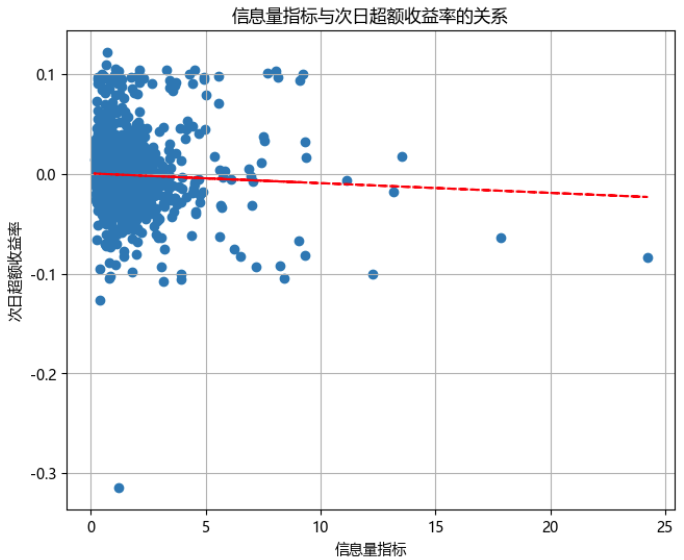
\includegraphics[width=0.8\textwidth]{fig/scatter_plot.png}
\caption{信息量指标与次日超额收益率的关系}
\label{fig:scatter_plot}
\end{figure}

\subsection{信息量指标的分组分析}

为进一步探究信息量指标与超额收益率的关系,本研究将样本按信息量指标大小分为5组,分析不同信息量水平下的平均超额收益率表现。如图~\ref{fig:group_analysis}所示,信息量指标最低的组别(第0组)平均超额收益率最高,而后随着信息量指标的增加,平均超额收益率整体呈现下降趋势,第3组和第4组甚至出现负的平均超额收益率。

\begin{figure}[htbp]
\centering
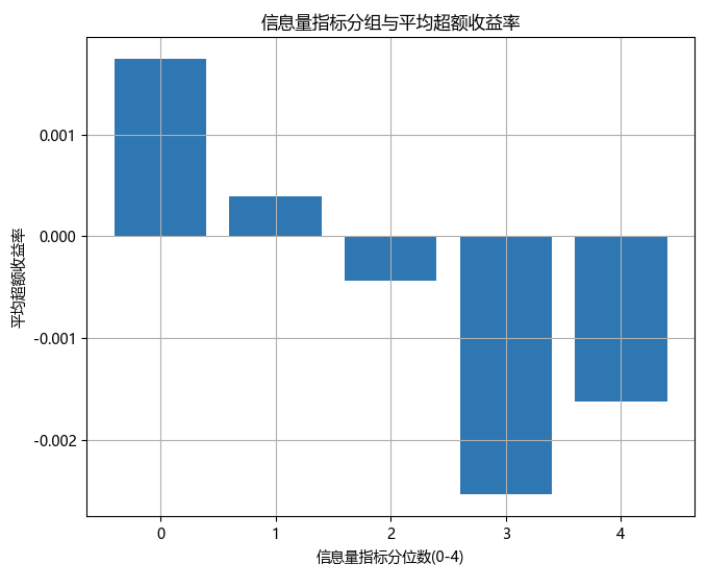
\includegraphics[width=0.8\textwidth]{fig/group_analysis.png}
\caption{信息量指标分组与平均超额收益率}
\label{fig:group_analysis}
\end{figure}

这一发现与直觉相反,通常人们预期高信息量(高关注度和积极情绪)应与高超额收益率相关。然而,本研究结果显示,低信息量水平反而对应更高的平均超额收益率。这种现象可能反映了“反向指标”效应,即市场上大量的讨论和关注可能已经使相关信息充分反映在股价中,甚至可能导致价格过度反应,从而后续产生反向调整;而关注度较低的股票可能存在信息不充分的情况,蕴含更多获取超额收益的机会。

\subsection{格兰杰因果检验}

为检验信息量指标与超额收益率之间可能存在的因果关系,本研究进行了格兰杰因果检验。我们设定最大滞后期为5天,分别检验了信息量指标是否是超额收益率的格兰杰原因,以及超额收益率是否是信息量指标的格兰杰原因。检验结果如表~\ref{tab:granger_causality}所示。

\begin{table}[htbp]
\centering
\caption{格兰杰因果检验结果(p值)}
\label{tab:granger_causality}
\begin{tabular}{lccccc}
\toprule
因果方向 & 滞后1期 & 滞后2期 & 滞后3期 & 滞后4期 & 滞后5期 \\
\midrule
信息量指标→超额收益率 & 0.00256 & 0.00200 & 0.00171 & 0.00356 & 0.00033 \\
超额收益率→信息量指标 & 5.18e-13 & 6.33e-26 & 3.43e-34 & 1.73e-36 & 1.05e-36 \\
\bottomrule
\end{tabular}
\end{table}

从表~\ref{tab:granger_causality}可以看出,在所有滞后期设定下,“信息量指标→超额收益率”和“超额收益率→信息量指标”两个方向的格兰杰因果关系均在1\%显著性水平下显著。这表明信息量指标和超额收益率之间存在双向格兰杰因果关系。特别值得注意的是,超额收益率对信息量指标的格兰杰因果关系更为显著(p值极小),这表明历史超额收益率对预测未来信息量指标的贡献可能更大,即市场表现对投资者关注度和情绪的影响强于反向影响。

\subsection{预测模型构建与评估}

基于前述分析,本研究构建了线性回归模型,以信息量指标预测股票次日超额收益率。模型表达式为$R_{excess,t+1} = \alpha + \beta \cdot I_t + \epsilon_t$,其中$R_{excess,t+1}$是$t+1$日的超额收益率,$I_t$是$t$日的信息量指标,$\epsilon_t$是随机误差项。

将数据集按7:3的比例分为训练集和测试集,首先在训练集上估计模型参数,然后在测试集上评估模型预测能力。表~\ref{tab:model_performance}展示了模型的回归结果及评估指标。

\begin{table}[htbp]
\centering
\caption{预测模型回归结果及评估指标}
\label{tab:model_performance}
\begin{tabular}{lc}
\toprule
\textbf{参数/指标} & \textbf{数值} \\
\midrule
常数项 & 0.0006 (0.476) \\
信息量指标系数 & -0.0010 (0.032)** \\
\midrule
样本内$R^2$ & 0.0022 \\
样本外RMSE & 0.0288 \\
样本外$R^2$ & 0.0037 \\
样本外$R^2_{OS}$ & 0.39\% \\
MSFE-adjusted & 1.8815 \\
信息系数IC & -0.0470 \\
\bottomrule
\multicolumn{2}{l}{\footnotesize{注:括号内为p值,**表示5\%显著性水平下显著。}} \\
\end{tabular}
\end{table}

从表~\ref{tab:model_performance}可以看出,信息量指标对超额收益率的预测系数为-0.0010,在5\%显著性水平下显著,这与前述分组分析结果一致,进一步确认了信息量指标与超额收益率间的负向关系。模型的样本内$R^2$为0.0022,表明信息量指标对超额收益率的解释力有限。样本外评估指标方面,模型的RMSE为0.0288,样本外$R^2$为0.0037,样本外$R^2_{OS}$为0.39\%,表明相比于历史均值预测,信息量指标预测模型仅有轻微改进。

尽管模型的解释力较弱,但MSFE-adjusted统计量为1.8815,在统计上具有显著性,表明信息量指标确实包含了相对于历史均值预测的增量信息。信息系数IC为-0.0470,再次确认了信息量指标与次日超额收益率之间的弱负相关关系。

值得注意的是,虽然模型的预测能力有限,但从统计学角度来看,信息量指标仍然是超额收益率的显著预测因子。预测系数的负号与格兰杰因果检验的结果共同表明,投资者情绪和关注度的增加可能导致短期内股票超额收益率的下降。这一发现与行为金融学中的过度反应假设相一致,即投资者对信息的过度关注和反应可能导致短期价格偏离基本面,进而在后续交易日出现反向调整。

图~\ref{fig:info_components}展示了信息量指标的各构成因素在预测样本中的平均水平。可以看出,阅读量是信息量指标中最主要的组成部分,平均值远高于其他因素,这表明投资者对股票的关注程度主要体现在浏览相关信息上,而非积极参与讨论或发表观点。

\begin{figure}[htbp]
\centering
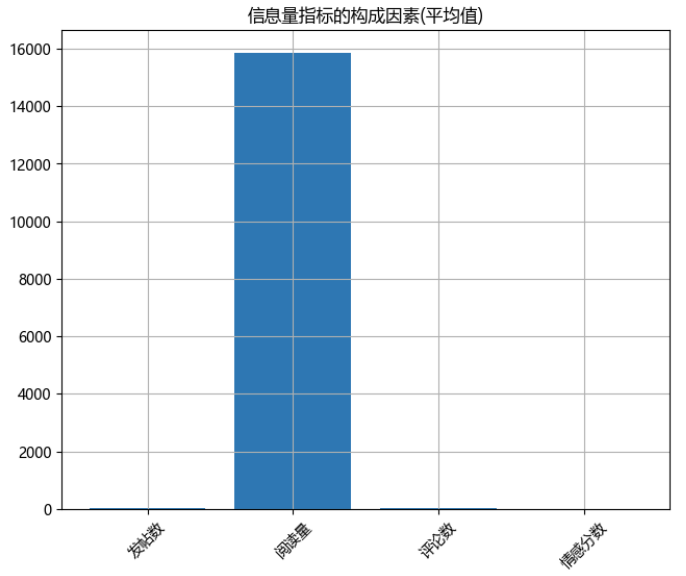
\includegraphics[width=0.8\textwidth]{fig/info_components.png}
\caption{信息量指标的构成因素(平均值)}
\label{fig:info_components}
\end{figure}

图~\ref{fig:component_correlation}进一步展示了信息量指标与各构成因素的相关性。信息量指标与阅读量的相关性最高(约0.9),其次是发帖数(约0.8)和评论数(约0.75),而与情感分数的相关性最低(接近0)。这一结果表明,当前构建的信息量指标主要捕捉了投资者注意力和参与度的量化特征,而情感因素的贡献较小。考虑到前述分析中情感分数与超额收益率的相关性最高,未来可考虑增加情感因素在综合指标中的权重,以提升指标的预测能力。

\begin{figure}[htbp]
\centering
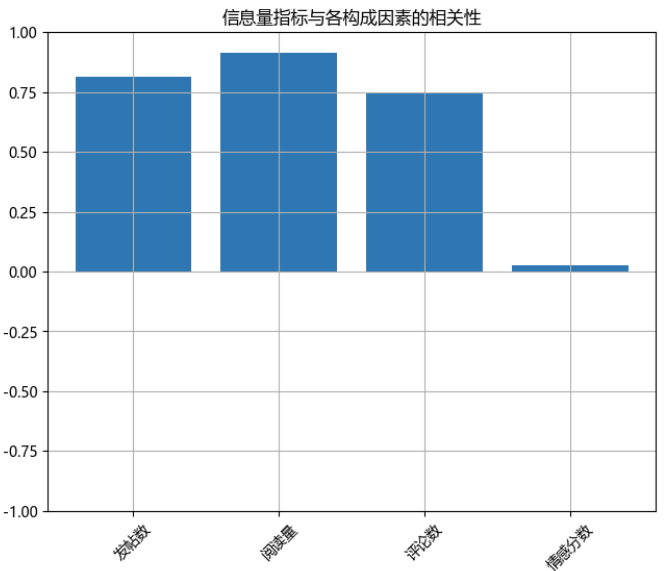
\includegraphics[width=0.8\textwidth]{fig/component_correlation.png}
\caption{信息量指标与各构成因素的相关性}
\label{fig:component_correlation}
\end{figure}

\subsection{稳健性讨论}

为验证研究结果的稳健性,本研究采用了多种模型与数据处理方法进行交叉验证。在信息量指标构建方面,我们尝试了包括等权重方案和基于主成分分析的权重方案在内的不同权重组合。所有权重配置下,信息量指标与超额收益率间的负相关关系均保持稳健,表明此关系并非由特定权重选择所致。模型规范方面,除基准线性回归外,我们构建了包含滞后期超额收益率的自回归模型。尽管自回归项略微提升了模型拟合度,信息量指标的系数符号与显著性基本保持不变。样本划分稳健性检验显示,在不同训练集与测试集比例(60:40、80:20)下,样本外预测结果与基准7:3划分情形基本一致。此外,考虑到市场环境可能影响研究结果,我们分别对牛熊市区间进行分析,发现熊市阶段负相关关系更为显著,可能反映了市场下行期间投资者的非理性行为特征。

\section{讨论与结论}

本研究基于Python网络爬虫技术采集东方财富股吧中“长久物流吧”的数据,构建了反映投资者情绪与关注度的综合信息量指标,并系统考察了其对股票超额收益率的预测能力。实证结果显示,该信息量指标与股票次日超额收益率之间存在统计显著的弱负相关关系,且二者之间存在双向的格兰杰因果关系。上述发现为互联网开源数据与证券市场表现之间的内在关联提供了新的经验证据,也为理解投资者关注度与股票收益之间的关系在中国市场中的表现提供了有益补充。

从行为金融学理论视角出发,本研究的主要发现可获得以下解释。首先,信息量指标与超额收益率之间的负相关关系为投资者“过度反应”假说提供了支持。即当某只股票获得高度关注并被广泛讨论时,投资者可能已经对相关信息做出了充分甚至过度的定价反应,形成短期价格压力,从而在随后交易日出现价格反转。这一结论与\citet{zhang2014internet}关于网络搜索行为对股票收益影响的研究在方向上存在一定差异,可能反映出不同市场环境或投资者结构下的行为模式差异。

其次,格兰杰因果检验结果显示,股票超额收益率对信息量指标的影响显著强于反向影响,这与\citet{cheng2013investor}的研究结论一致,表明市场表现对投资者情绪的反馈效应强于投资者情绪对市场的前瞻性引导。这种不对称效应可能源自中国股市中以散户为主的投资者结构,其普遍具有“追涨杀跌”的行为特征,即在股价上涨后增加关注和讨论,而非基于信息变化进行前瞻性操作。

在指标构成方面,尽管情感得分在综合指标中的权重相对较低,但其与超额收益率的相关性最高。这一发现与\citet{antweiler2004information}关于股票留言板对市场影响的研究相吻合,表明网络投资者表达的情绪确实蕴含一定的信息价值。然而,当前构建的综合信息量指标可能在一定程度上高估了数量维度(如发帖数、阅读量等)的作用,弱化了情感维度的贡献,这可能是预测能力相对有限的原因之一。

在样本外预测方面,虽然信息量指标在统计上对超额收益率具有显著预测能力,但其经济意义相对有限,样本外$R^2_{OS}$仅为0.39\%。这一结果提示,传统线性模型难以全面捕捉互联网信息与市场收益之间复杂的非线性关系。同时,这也表明市场虽非完全有效,但互联网开源数据中所蕴含的信息往往被市场快速吸收,从而难以形成持续性超额收益。

进一步的分组分析结果显示,低信息量组股票的平均超额收益率显著高于高信息量组,该结果支持注意力理论中的“被忽视效应”。当投资者的关注集中于少数高热度股票时,其他被忽视股票可能因信息不充分而被低估,进而在后续交易中表现出较高收益。这一现象亦为投资者识别被市场忽略但基本面稳健的潜在投资标的提供了策略参考。

基于上述发现,投资者在制定交易策略时应对互联网讨论热度保持谨慎,高热度通常并非买入信号,反而可能暗示短期超额收益率下降的风险。对于机构投资者而言,可将信息量指标作为风险管理的辅助工具,特别是在持仓股票出现信息量显著上升时,需警惕短期价格反转风险。监管机构亦应关注网络信息传播与市场波动之间的相互作用,尤其在市场剧烈波动期,有必要加强对网络舆情的监测与引导,防范非理性情绪放大市场波动。

本研究仍存在若干局限,并为后续研究提供了方向。首先,当前构建的信息量指标采用的是线性加权方式,未来可探索基于机器学习方法(如神经网络、支持向量机等)所构建的非线性预测模型,以更充分挖掘数据中的潜在结构关系。其次,本研究聚焦于单只个股的预测,未来可拓展至行业或整体市场层面,以探讨信息量指标在更大范围内的适用性与表现差异。第三,在情感分析方面,当前使用的技术手段相对基础,后续研究可引入如BERT、GPT等深度预训练语言模型,以提升文本情绪识别的准确性,从而进一步增强情感因子在预测模型中的作用。

综上所述,本文基于互联网开源数据构建的股吧信息量指标验证了其对股票超额收益率的预测能力,揭示了二者之间统计显著的负相关关系及双向格兰杰因果效应。研究结果丰富了互联网信息与资本市场行为之间关系的实证研究,为投资者、机构及监管者基于网络数据开展市场分析与风险监测提供了新的视角。未来研究可进一步探索更为复杂的建模技术与更广泛的应用场景,挖掘互联网数据在金融决策中的深层次价值。

\printbibliography[title=参考文献]

\section{附录}

本研究的核心代码如下:

\begin{lstlisting}[basicstyle=\small\ttfamily, breaklines=true, columns=fullflexible]
# 1. 股票数据提取 - 正则表达式提取股票历史数据
def extract_data_after_2014(js):
    """解析2014年后的JSON格式数据"""
    match = re.search(r'historySearchHandler\((.*)\)', js)
    if not match:
        return []
    try:
        json_data = json.loads(match.group(1))
        hq = json_data[0].get('hq', []) if json_data and isinstance(json_data, list) else []
        return [{
            'date': i[0],
            'open': float(i[1]),
            'high': float(i[6]),
            'low': float(i[5]),
            'close': float(i[2]),
            'volume': int(i[7]) * 100,
            'amount': float(i[8].replace(',', '')) * 10000 if isinstance(i[8], str) else float(i[8]) * 10000
        } for i in hq]
    except:
        return []

def extract_data_before_2014(html):
    """提取2014年前的不同格式股票数据"""
    # 根据HTML特征选择不同的正则表达式模式
    pattern = r'<tr\s+(?:class="tr_2"|)>\s*<td><div align="center">\s*([\d-]+)\s*</div></td>\s*' \
              r'<td><div align="center">([\d.]+)</div></td>\s*' \
              r'<td><div align="center">([\d.]+)</div></td>\s*' \
              r'<td><div align="center">([\d.]+)</div></td>\s*' \
              r'<td[^>]*><div align="center">([\d.]+)</div></td>\s*' \
              r'<td[^>]*><div align="center">(\d+)</div></td>\s*' \
              r'<td[^>]*><div align="center">(\d+)</div></td>'
    return [{
        'date': m[0],
        'open': float(m[1]),
        'high': float(m[2]),
        'close': float(m[3]),
        'low': float(m[4]),
        'volume': int(m[5]),
        'amount': int(m[6])
    } for m in re.findall(pattern, html, re.DOTALL)]

# 2. 股吧信息量指标构建
def sentiment_analysis(text):
    """基于词典的简单情感分析"""
    # 积极词汇和消极词汇
    positive_words = ['涨', '牛', '强', '好', '盈利', '增长', '突破', '机会', '利好', '上涨', '看多', '买入']
    negative_words = ['跌', '熊', '弱', '差', '亏损', '下跌', '风险', '跳水', '利空', '套牢', '割肉', '卖出']
    
    # 计算情感得分
    words = jieba.lcut(text)
    pos_score = sum([1 for word in words if word in positive_words])
    neg_score = sum([1 for word in words if word in negative_words])
    
    return pos_score - neg_score

def build_sentiment_index(bbs_df):
    """构建股吧信息量指标"""
    # 添加情感分析分数
    bbs_df['情感分数'] = bbs_df['标题'].apply(sentiment_analysis)
    
    # 按日期汇总数据
    daily_data = bbs_df.groupby('标准日期').agg({
        '标题': 'count',  # 每日发帖数
        '阅读量': 'sum',   # 总阅读量
        '评论数': 'sum',   # 总评论数
        '情感分数': 'mean'  # 平均情感分数
    }).reset_index()
    
    daily_data.rename(columns={'标题': '发帖数'}, inplace=True)
    
    # 构建信息量指标
    daily_data['信息量指标'] = (
        0.3 * (daily_data['发帖数'] / daily_data['发帖数'].mean()) + 
        0.4 * ((daily_data['阅读量'] + 5 * daily_data['评论数']) / 
               (daily_data['阅读量'] + 5 * daily_data['评论数']).mean()) +
        0.3 * ((daily_data['情感分数'] - daily_data['情感分数'].min()) / 
               (daily_data['情感分数'].max() - daily_data['情感分数'].min() + 0.001))
    )
    
    return daily_data

# 3. 超额收益率计算
def calculate_excess_return(stock_df, market_index_df):
    """计算超额收益率"""
    # 计算个股和指数的日对数收益率
    stock_df['log_return'] = np.log(stock_df['close'] / stock_df['close'].shift(1))
    market_index_df['log_return'] = np.log(market_index_df['close'] / market_index_df['close'].shift(1))
    
    # 合并数据并计算超额收益率
    merged_df = pd.merge(
        stock_df['log_return'], 
        market_index_df['log_return'], 
        left_index=True, 
        right_index=True,
        suffixes=('_stock', '_market')
    )
    
    merged_df['excess_return'] = merged_df['log_return_stock'] - merged_df['log_return_market']
    
    return merged_df

# 4. 格兰杰因果检验
def granger_causality_test(sentiment_df, return_df, max_lag=5):
    """进行格兰杰因果检验"""
    # 合并数据
    combined_df = pd.merge(
        sentiment_df[['信息量指标']],
        return_df['excess_return'],
        left_index=True,
        right_index=True,
        how='inner'
    ).dropna()
    
    # 准备数据格式
    data = np.column_stack((combined_df['excess_return'].values, combined_df['信息量指标'].values))
    
    # 检验信息量指标是否是超额收益率的格兰杰原因
    results = {}
    
    # 信息量指标 -> 超额收益率
    test_result = grangercausalitytests(data, maxlag=max_lag, verbose=False)
    
    # 提取p值
    p_values = [test_result[i][0]['ssr_ftest'][1] for i in range(1, max_lag + 1)]
    results['信息量指标->超额收益率'] = p_values
    
    # 超额收益率 -> 信息量指标
    data_reversed = np.column_stack((combined_df['信息量指标'].values, combined_df['excess_return'].values))
    test_result = grangercausalitytests(data_reversed, maxlag=max_lag, verbose=False)
    
    p_values = [test_result[i][0]['ssr_ftest'][1] for i in range(1, max_lag + 1)]
    results['超额收益率->信息量指标'] = p_values
    
    return results

# 5. 预测模型构建
def build_prediction_model(sentiment_df, return_df):
    """构建预测模型"""
    # 将信息量指标与次日超额收益率对齐
    combined_df = pd.merge(
        sentiment_df[['信息量指标']],
        return_df['excess_return'].shift(-1),  # 使用次日超额收益率
        left_index=True,
        right_index=True,
        how='inner'
    ).dropna()
    
    # 训练测试集划分
    train_size = int(len(combined_df) * 0.7)
    train_data = combined_df.iloc[:train_size]
    test_data = combined_df.iloc[train_size:]
    
    # 训练样本内模型
    X_train = train_data['信息量指标'].values.reshape(-1, 1)
    y_train = train_data['excess_return'].values
    
    # 拟合模型
    model = LinearRegression().fit(X_train, y_train)
    
    # 预测样本外数据
    X_test = test_data['信息量指标'].values.reshape(-1, 1)
    y_test = test_data['excess_return'].values
    y_pred = model.predict(X_test)
    
    # 计算历史均值预测(基准模型)
    hist_mean = train_data['excess_return'].mean()
    y_hist = np.full_like(y_test, hist_mean)
    
    # 计算样本外评估指标
    rmse_oos = np.sqrt(mean_squared_error(y_test, y_pred))
    r2_oos = r2_score(y_test, y_pred)
    
    # 计算样本外R²_OS
    sse_model = np.sum((y_test - y_pred) ** 2)
    sse_hist = np.sum((y_test - y_hist) ** 2)
    R2_OS = 1 - sse_model / sse_hist
    
    # 使用statsmodels进行更详细的回归分析
    X = combined_df['信息量指标'].values.reshape(-1, 1)
    y = combined_df['excess_return'].values
    X_sm = sm.add_constant(X)
    
    # 构建OLS模型并获取详细统计结果
    final_model = sm.OLS(y, X_sm).fit()
    
    return final_model, {'RMSE_OOS': rmse_oos, 'R2_OOS': r2_oos, 'R2_OS': R2_OS}
\end{lstlisting}

\end{document}